\documentclass[a4paper, 12pt]{article}

\usepackage{cmap}
\usepackage[T2A]{fontenc}
\usepackage[utf8]{inputenc}
\usepackage{amsmath}
\usepackage{mathtools}
\usepackage[english, russian]{babel}
\usepackage{graphicx}
\graphicspath{{../img/}}

\usepackage{geometry}
\geometry{right=20mm}
\geometry{left=20mm}
\geometry{top=20mm}
\geometry{bottom=20mm}

\usepackage{pythontex}

\begin{document}
    \section{Сканер}

    \subsection{Формулы}

    \subsubsection{Основные определения}
    
    Рабочая плоскость --- плоскость перпендикулярная оптической оси камеры и проходящая через точку пересечения оптической оси камеры и луча лазера\\
    Измеряемая плоскость --- плоскость, до которой измеряется расстояние\\
    Начальная плоскость --- плоскость, координата $z$ которой в глобальной СК равна нулю\\
    $\prescript{k}{}{X} \prescript{k}{}{Y} \prescript{k}{}{Z}$ --- система координат камеры\\
    $(\prescript{k}{}{x} \prescript{k}{}{y} \prescript{k}{}{z})$ --- координата точки в СК камеры\\
    $f$ --- фокусное расстояние камеры\\
    $H$ --- расстояние от оптического центра камеры до рабочей плоскости; рабочая высота сканера\\
    $\alpha$ --- угол между оптической осью камеры и лучём лазера\\
    $\beta$ --- угол отклонения отраженного луча лазера от оптической оси камеры в плоскости $\prescript{k}{}{Z}\prescript{k}{}{Y}$\\
    $\gamma$ --- угол отклонения отраженного луча лазера от оптической оси камеры в плоскости $\prescript{k}{}{Z}\prescript{k}{}{X}$\\
    $\Delta x$ --- отклонение лазера от оптического центра на изображении по оси $X$\\
    $\Delta y$ --- отклонение лазера от оптического центра на изображении по оси $Y$\\
    $\tg\beta = \dfrac{\Delta y}{f}$ --- тангенс угла отклонения лазера в плоскости $\prescript{k}{}{Z}\prescript{k}{}{Y}$\\
    $\tg\gamma = \dfrac{\Delta x}{f}$ --- тангенс угла отклонения лазера в плоскости $\prescript{k}{}{Z}\prescript{k}{}{X}$\\

    \subsubsection{Основные формулы}
    \begin{equation}
        \label{eq:camcoord_pixel}
        \begin{aligned}
            \prescript{k}{}{x}_p = H\frac{\tg\alpha\frac{\Delta x}{f}}{\tg\alpha+\frac{\Delta y}{f}}\\
            \prescript{k}{}{y}_p = H\frac{\tg\alpha\frac{\Delta y}{f}}{\tg\alpha+\frac{\Delta y}{f}}\\
            \prescript{k}{}{z}_p = H\frac{\tg\alpha}{\tg\alpha+\frac{\Delta y}{f}}
        \end{aligned}
    \end{equation}
    Уравнение\footnote{Вывод уравнений на странице~\pageref{subsec:вывод_формул} в разделе~\ref{subsec:вывод_формул}}~\eqref{eq:camcoord_pixel} позволяет рассчитать координаты точки в СК камеры через отклонение лазера на изображении.
    При этом $\Delta x$, $\Delta y$ и $f$ должны быть выражены в одних единицах - пиксели или миллиметры.

    \begin{equation}
        \label{eq:coord_world}
        \begin{pmatrix}
            x\\y\\z
        \end{pmatrix}
        =
        R
        \begin{pmatrix}
            \prescript{k}{}{x}_p\\
            \prescript{k}{}{x}_p\\
            \prescript{k}{}{x}_p
        \end{pmatrix}
        +
        \begin{pmatrix}
            x_k\\y_k\\z_k
        \end{pmatrix}
    \end{equation}
    Уравнение~\eqref{eq:coord_world} позволяет рассчитать координаты точки в глобальной СК зная матрицу поворота $R$ и координаты камеры в глобальной СК $x_k,\,y_k,\,z_k$

    \begin{equation}
        \label{eq:calibration}
        \left\{
        \begin{aligned}
            \tg\alpha &= \frac{h_k\tg\beta_k(\tg\beta_i-\tg\beta_0) - h_i\tg\beta_i(\tg\beta_k-\tg\beta_0)}{h_i(\tg\beta_k-\tg\beta_0) - h_k(\tg\beta_i-\tg\beta_0)}\\
            H &= h_i\frac{(\tg\alpha + \tg\beta_i)(\tg\alpha + \tg\beta_0)}{(\tg\beta_i - \tg\beta_0)(r_{32}\tg^2\alpha-r_{33}\tg\alpha)}
        \end{aligned}
        \right.
    \end{equation}
    Система уравнений~\eqref{eq:calibration} позволяет найти параметры сканера - рабочую высоту $H$ и угол $\alpha$ - зная высоты измеряемых объектов $h_i,\,h_k$, углы отклонения лазера $\beta_i,\,\beta_k$, соответствующих этим высотам, и угол отклонения луча от начальной плоскости

    \subsection{Устройство сканера}
    \begin{figure}[h!]
        \begin{center}
            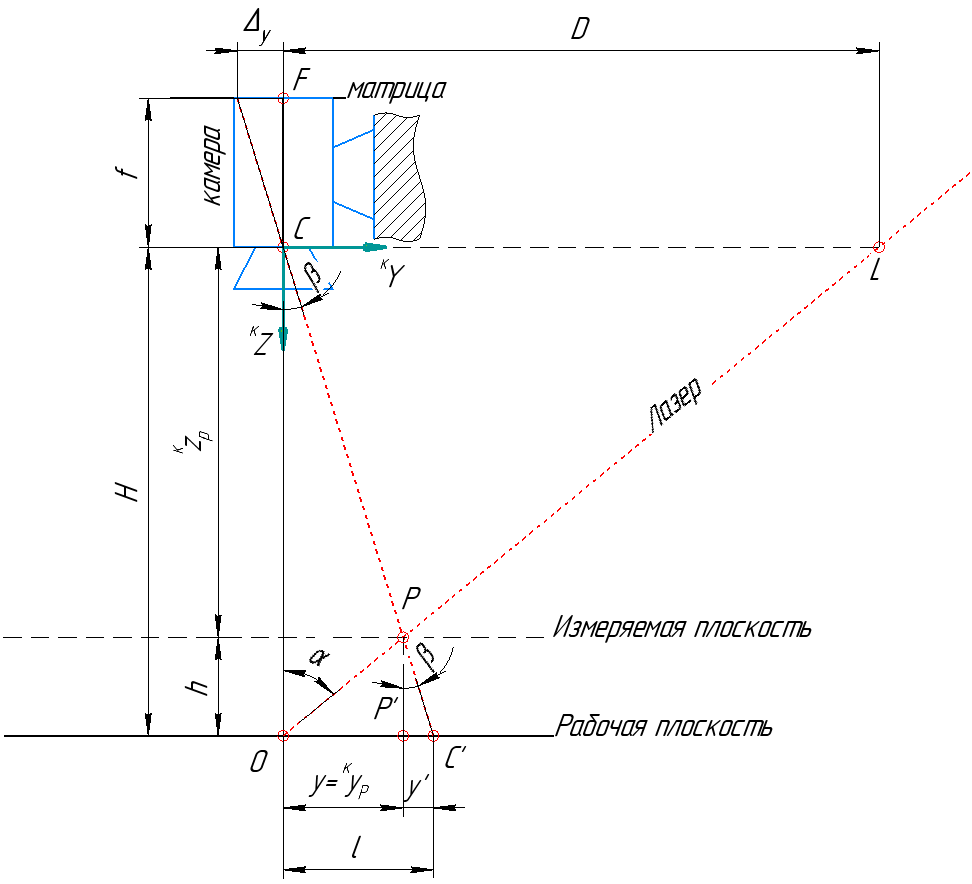
\includegraphics[width=0.75\linewidth]{main-scheme.png}
            \caption{Схема сканера}
        \end{center}
        
        $O$ --- точка пересечения оптической оси камеры и луча лазера (плоскости свечения лазера)\\
        $C$ --- оптический центр камеры, начало координат СК камеры\\
        $P$ --- точка пересечения луча лазера и измеряемой плоскости\\
        $P'$ --- проекция точки P на рабочую плоскость\\
        $h$ --- высота измеряемой плоскости над рабочей плоскостью\\
        $l_x,\,l_y$ --- кажущиеся координаты измеряемой точки\\
        $x,\,y$ --- реальные координаты измеряемой точки\\
        $x',\,y'$ --- разность кажущейся и реальной координаты измеряемой точки\\
    \end{figure}

    \subsection{Вывод формул}\label{subsec:вывод_формул}

    \subsubsection{Формулы расчёта координат в СК камеры}
    \begin{equation*}
        \begin{split}
            &\left\{
            \begin{aligned}
                l &= H \tg \beta \\
                l &= y + y'\\
            \end{aligned}
            \right.\\
            &\left\{
            \begin{aligned}
                l &= H \tg \beta \\
                l &= h \tg \alpha + h\tg\beta\\
            \end{aligned}
            \right.\\
            &\left\{
            \begin{aligned}
                l &= H \tg \beta \\
                l &= h(\tg\alpha+\tg\beta)\\
            \end{aligned}
            \right.\\
        \end{split}
    \end{equation*}
    \begin{equation*}
        \begin{split}
            h(\tg\alpha+\tg\beta)&=H\tg\beta\\
            h &= H\dfrac{\tg\beta}{\tg\alpha+\tg\beta}\\
        \end{split}
    \end{equation*}
    \begin{equation*}
        \begin{split}
            \prescript{k}{}{z}_p &= H-h = H(1-\frac{\tg\beta}{\tg\alpha+\tg\beta}) = H\dfrac{\tg\alpha}{\tg\alpha+\tg\beta}\\
            \prescript{k}{}{x}_p &= (H-h)\tg\gamma = z\tg\gamma = H\dfrac{\tg\alpha\tg\gamma}{\tg\alpha+\tg\beta}\\
            \prescript{k}{}{y}_p &= h\tg\alpha = z\tg\beta = H\dfrac{\tg\alpha\tg\beta}{\tg\alpha+\tg\beta}
        \end{split}
    \end{equation*}
    \begin{equation*}
        \label{eq:camcoord}
        \boxed{
            \begin{aligned}
                \prescript{k}{}{x}_p = H\frac{\tg\alpha\tg\gamma}{\tg\alpha+\tg\beta} = H\frac{\tg\alpha\frac{\Delta x}{f}}{\tg\alpha+\frac{\Delta y}{f}}\\
                \prescript{k}{}{y}_p = H\frac{\tg\alpha\tg\beta}{\tg\alpha+\tg\beta} = H\frac{\tg\alpha\frac{\Delta y}{f}}{\tg\alpha+\frac{\Delta y}{f}}\\
                \prescript{k}{}{z}_p = H\frac{\tg\alpha}{\tg\alpha+\tg\beta} = H\frac{\tg\alpha}{\tg\alpha+\frac{\Delta y}{f}}
            \end{aligned}
        }
    \end{equation*}

    \subsubsection{Формулы определения параметров сканера}
    \[
        \begin{pmatrix}
            x\\y\\z
        \end{pmatrix}
        =
        \begin{pmatrix}
            r_{11} & r_{12} & r_{13}\\
            r_{21} & r_{22} & r_{23}\\
            r_{31} & r_{32} & r_{33}
        \end{pmatrix}
        \begin{pmatrix}
            \prescript{k}{}{x}_p\\
            \prescript{k}{}{y}_p\\
            \prescript{k}{}{z}_p
        \end{pmatrix}
        +
        \begin{pmatrix}
            x_k\\y_k\\z_k
        \end{pmatrix}
    \]
    \[
        \begin{pmatrix}
            x\\y\\z
        \end{pmatrix}
        =
        \begin{pmatrix}
            r_{11} & r_{12} & r_{13}\\
            r_{21} & r_{22} & r_{23}\\
            r_{31} & r_{32} & r_{33}
        \end{pmatrix}
        \begin{pmatrix}
            \prescript{k}{}{z}_p\tg\gamma\\
            \prescript{k}{}{z}_p\tg\beta\\
            \prescript{k}{}{z}_p
        \end{pmatrix}
        +
        \begin{pmatrix}
            x_k\\y_k\\z_k
        \end{pmatrix}
    \]
    \[
        \begin{pmatrix}
            x\\y\\z
        \end{pmatrix}
        =
        \prescript{k}{}{z}_p
        \begin{pmatrix}
            r_{11}\tg\gamma + r_{12}\tg\beta + r_{13} + \frac{x_k}{\prescript{k}{}{z}_p}\\
            r_{21}\tg\gamma + r_{22}\tg\beta + r_{23} + \frac{y_k}{\prescript{k}{}{z}_p}\\
            r_{31}\tg\gamma + r_{32}\tg\beta + r_{33} + \frac{z_k}{\prescript{k}{}{z}_p}
        \end{pmatrix}
    \]
    \[
        \begin{split}
            x = \prescript{k}{}{z}_p(r_{11}\tg\gamma + r_{12}\tg\beta + r_{13}) + x_k\\
            y = \prescript{k}{}{z}_p(r_{21}\tg\gamma + r_{22}\tg\beta + r_{23}) + y_k\\
            z = \prescript{k}{}{z}_p(r_{31}\tg\gamma + r_{32}\tg\beta + r_{33}) + z_k\\
        \end{split}
    \]
    Пусть высота измеряемого объекта равна $h_i = z_i - z_0$, где $z_0$ это $z$ координата плоскости на которой лежит объект, $z_i$ это $z$ координата объекта.
    \[
        \begin{split}
            z_i &= \prescript{k}{}{z}_i(r_{31}\tg\gamma_i + r_{32}\tg\beta_i + r_{33}) + z_k\\
            z_i &= H\frac{\tg\alpha}{\tg\alpha+\tg\beta_i}(r_{31}\tg\gamma_i + r_{32}\tg\beta_i + r_{33}) + z_k\\
            z_i &= H\frac{\tg\alpha\tg\gamma_i}{\tg\alpha+\tg\beta_i}r_{31} + H\frac{\tg\alpha\tg\beta_i}{\tg\alpha+\tg\beta_i}r_{32} + H\frac{\tg\alpha}{\tg\alpha+\tg\beta_i}r_{33} + z_k
        \end{split}
    \]
    \[
        \begin{split}
            h_i = &\left(H\frac{\tg\alpha\tg\gamma_i}{\tg\alpha+\tg\beta_i}r_{31} + H\frac{\tg\alpha\tg\beta_i}{\tg\alpha+\tg\beta_i}r_{32} + H\frac{\tg\alpha}{\tg\alpha+\tg\beta_i}r_{33}\right)-\\
            - &\left(H\frac{\tg\alpha\tg\gamma_0}{\tg\alpha+\tg\beta_0}r_{31} + H\frac{\tg\alpha\tg\beta_0}{\tg\alpha+\tg\beta_0}r_{32} + H\frac{\tg\alpha}{\tg\alpha+\tg\beta_0}r_{33}\right)
        \end{split}
    \]
    \[
        \begin{aligned}
            h_i = r_{31} H \tg\alpha &\left(\frac{\tg\gamma_i}{\tg\alpha+\tg\beta_i} - \frac{\tg\gamma_0}{\tg\alpha+\tg\beta_0}\right)+\\
            + r_{32} H \tg\alpha &\left(\frac{\tg\beta_i}{\tg\alpha+\tg\beta_i} - \frac{\tg\beta_0}{\tg\alpha+\tg\beta_0}\right)+\\
            + r_{33} H \tg\alpha &\left(\frac{1}{\tg\alpha+\tg\beta_i} - \frac{1}{\tg\alpha+\tg\beta_0}\right)
        \end{aligned}
    \]
    \[
        \begin{aligned}
            h_i = &r_{31} H \tg\alpha \left(\frac{\tg\gamma_i}{\tg\alpha+\tg\beta_i} - \frac{\tg\gamma_0}{\tg\alpha+\tg\beta_0}\right)+\\
            + &r_{32} H \tg\alpha \frac{\tg\beta_i(\tg\alpha+\tg\beta_0)-\tg\beta_0(\tg\alpha+\tg\beta_i)}{(\tg\alpha+\tg\beta_i)(\tg\alpha+\tg\beta_0)}+\\
            + &r_{33} H \tg\alpha \frac{\tg\beta_0 - \tg\beta_i}{(\tg\alpha+\tg\beta_i)(\tg\alpha+\tg\beta_0)}
        \end{aligned}
    \]
    Пусть $\tg\gamma_0$ и $\tg\gamma_i$ равны нулю, т.е. объект находится посередине кадра, тогда
    \begin{gather*}
        h_i = r_{32} H \tg\alpha \frac{\tg\alpha(\tg\beta_i -\tg\beta_0)}{(\tg\alpha+\tg\beta_i)(\tg\alpha+\tg\beta_0)}
        - r_{33} H \tg\alpha \frac{\tg\beta_i - \tg\beta_0}{(\tg\alpha+\tg\beta_i)(\tg\alpha+\tg\beta_0)}\\
        h_i = H\tg\alpha\frac{\tg\beta_i-\tg\beta_0}{(\tg\alpha+\tg\beta_i)(\tg\alpha+\tg\beta_0)}(r_{32}\tg\alpha-r_{33})\\
    \end{gather*}
    Имея минимум два объекта известной высоты можем решить систему уравнений и найти $H$ и $\tg\alpha$
    \begin{equation*}
        \left\{
        \begin{aligned}
            h_i &= H\tg\alpha\frac{\tg\beta_i - \tg\beta_0}{(\tg\alpha + \tg\beta_i)(\tg\alpha + \tg\beta_0)}(r_{32}\tg\alpha-r_{33})\\
            h_k &= H\tg\alpha\frac{\tg\beta_k - \tg\beta_0}{(\tg\alpha + \tg\beta_k)(\tg\alpha + \tg\beta_0)}(r_{32}\tg\alpha-r_{33})
        \end{aligned}
        \right.
    \end{equation*}
    \begin{gather*}
        \frac{h_i}{h_k} = \frac{(\tg\beta_i - \tg\beta_0)(\tg\alpha + \tg\beta_k)}{(\tg\beta_k - \tg\beta_0)(\tg\alpha + \tg\beta_i)}\\
        \frac{h_i}{h_k} = \frac{\tg\alpha(\tg\beta_i-\tg\beta_0) + \tg\beta_k(\tg\beta_i-\tg\beta_0)}{\tg\alpha(\tg\beta_k-\tg\beta_0) + \tg\beta_i(\tg\beta_k-\tg\beta_0)}\\
        h_i(\tg\alpha(\tg\beta_k-\tg\beta_0) + \tg\beta_i(\tg\beta_k-\tg\beta_0)) =
        h_k(\tg\alpha(\tg\beta_i-\tg\beta_0) + \tg\beta_k(\tg\beta_i-\tg\beta_0))\\
        h_i\tg\alpha(\tg\beta_k-\tg\beta_0) - h_k\tg\alpha(\tg\beta_i-\tg\beta_0) =
        h_k\tg\beta_k(\tg\beta_i-\tg\beta_0) - h_i\tg\beta_i(\tg\beta_k-\tg\beta_0)\\
        \tg\alpha(h_i(\tg\beta_k-\tg\beta_0) - h_k(\tg\beta_i-\tg\beta_0)) =
        h_k\tg\beta_k(\tg\beta_i-\tg\beta_0) - h_i\tg\beta_i(\tg\beta_k-\tg\beta_0)\\
    \end{gather*}
    \[
        \tg\alpha =
        \frac{h_k\tg\beta_k(\tg\beta_i-\tg\beta_0) - h_i\tg\beta_i(\tg\beta_k-\tg\beta_0)}{h_i(\tg\beta_k-\tg\beta_0) - h_k(\tg\beta_i-\tg\beta_0)} \eqno (*)
    \]
    Уравнение (*) позволяет найти $\tg\alpha$ при известных значениях высот объектов $h_i,\,h_k$, углах отклонения лазера $\beta_i,\,\beta_k$, соответствующих этим высотам, и угла отклонения луча от начальной плоскости. Подставив таким образом получившееся значение в систему уравнений, можно найти рабочую высоту $H$ сканера.
    \begin{equation*}
        \boxed{
            \left\{
            \begin{aligned}
                \tg\alpha &= \frac{h_k\tg\beta_k(\tg\beta_i-\tg\beta_0) - h_i\tg\beta_i(\tg\beta_k-\tg\beta_0)}{h_i(\tg\beta_k-\tg\beta_0) - h_k(\tg\beta_i-\tg\beta_0)}\\
                H &= h_i\frac{(\tg\alpha + \tg\beta_i)(\tg\alpha + \tg\beta_0)}{(\tg\beta_i - \tg\beta_0)(r_{32}\tg^2\alpha-r_{33}\tg\alpha)}
            \end{aligned}
            \right.
        }
    \end{equation*}


\end{document}
